\chapter[What Kind of Chemical System Is Life?]{What Kind of Chemical\protect\\ System Is Life?}

\begin{kaichang}
Take a handful of dried mung beans, spread them on wet gauze, and sprinkle them with water every day. On the third day, the beans split and tender white roots emerge; on the fifth day, they have become a stand of upright bean sprouts.

Now think carefully about a question: which is more ``disordered''---the handful of dried beans or these sprouts?

Your intuition might say: the dried beans were heaped together haphazardly, but the sprouts have their roots pointing down and their shoots pointing up, neatly arranged and developing intricate structures. The sprouts are clearly more ``ordered.'' Yet in Chapter 28 we just encountered an ironclad rule: in an isolated system, every process increases entropy; everything moves toward greater disorder, never spontaneously toward greater order. A bean soaking in water has no designer and no blueprint. How can it grow increasingly elaborate?

Is it an exception to the laws of nature? Write down your guess first. We will return to check it at the end of this chapter---and after this chapter, you will officially cross from ``chemistry'' into ``life.''
\end{kaichang}

\section{First, Look at What Is Right Before Us}

Before offering any theory, let us lay out the facts we can see, touch, and measure with a thermometer. Compare living and nonliving things, and the differences are plain:

\begin{itemize}[itemsep=2pt]
\item Bean sprouts grow taller and heavier every day, their structures becoming increasingly complex; a glass marble in the same tray would remain unchanged for ten thousand years.
\item A bowl of cooked rice turns sour after two days---something invisible is ``eating'' it; thoroughly sterilized, vacuum-packed canned food can last for years.
\item Even when you sit quietly, your body temperature stays close to $37\,^{\circ}\mathrm{C}$, much the same in winter and summer; a stone simply settles at the temperature of its surroundings.
\item A cut on your hand heals by itself in a few days; a cut in a sweater only grows larger.
\item Fallen autumn leaves return to the soil and ``disappear'' after a few years---invisible things have dismantled them into raw materials again.
\end{itemize}

\textbf{Translator safety note:} Do not seal an animal in a container to reproduce the example below. Use published measurements or a teacher-reviewed non-animal demonstration; student activities must protect animals from distress and provide suitable ventilation. See \href{https://www.societyforscience.org/isef/international-rules/vertebrate-animals/}{Society for Science's animal-welfare rules}.

These phenomena are measurable, too: place a small animal (or a germinating seed) in a sealed container, and oxygen decreases, carbon dioxide increases, and the thermometer rises slightly. Living things continuously ``take in'' and ``give out'' something, while continuously producing heat. This is life's most conspicuous feature: \textbf{it is not a thing, but an uninterrupted flow}.

\textbf{Translator safety note:} Do not sniff, taste, or handle moldy beans to check the observations below, and do not eat either experimental batch. Have an adult discard moldy material in a closed bag and clean the container. See \href{https://www.fsis.usda.gov/food-safety/safe-food-handling-and-preparation/food-safety-basics/molds-food-are-they-dangerous}{USDA mold-handling guidance}.

\begin{shiyan}
\textbf{Grow a Tray of Bean Sprouts and Watch Life ``Get to Work''}

Materials: a small handful of dried mung beans, a shallow tray or draining basket, clean gauze or paper towels, clean water, a thermometer (optional), and kitchen scales (optional).

Steps:
\begin{enumerate}[itemsep=1pt]
\item Take two equal portions of dried mung beans (for example, \ud{20}{g} each). Boil one portion and let it cool as a control; leave the other raw.
\item Spread them in separate shallow trays lined with wet gauze, label them ``raw'' and ``cooked,'' and keep them at room temperature away from light.
\item Sprinkle with water and observe at the same time each day for 5--7 days. Record whether the beans swell, split their skins and sprout roots, and whether the gauze develops an odor. If you have scales, track the change in wet mass; if you have a thermometer, bury it among the beans for a few minutes and compare the two trays' temperatures.
\end{enumerate}

What to observe: the raw beans absorb water, swell, split, root, and sprout. After a few days, the tray becomes slightly warm during vigorous germination. The boiled portion only gradually becomes slimy and moldy. Think about it: what is the mold? It, too, is ``getting to work''---just on a different job.

Safety note: this is a safe home observation. Wash your hands frequently; do not taste moldy beans. Discard them and clean the container.
\end{shiyan}

\section{Zooming In on the Cell}

Why do bean sprouts move, grow, and produce heat? Zoom inward: every small section of a sprout consists of hundreds of millions of tiny ``rooms''---cells (Chapter 57 will take you on a room-by-room tour). A thin membrane surrounds each cell (Chapter 51 is devoted to this membrane). Inside is not a stagnant soup but a factory working day and night: nutrient molecules enter through the membrane, are broken down, modified, and reassembled, while waste and heat leave.

How enormous is the scale? An ordinary cell carries out millions of chemical reactions every second; the cells throughout your body synthesize trillions of protein molecules per second. None of this is a chaotic free-for-all: which molecule reacts with which partner, where, and when is precisely controlled. The dispatchers responsible for these reactions are enzymes, the subject of Chapter 49.

Return to the five questions that run through this book, now asking them about ``life'':

\begin{enumerate}[itemsep=2pt]
\item What is it made of?---Water, proteins, carbohydrates, lipids, and nucleic acids; ultimately, atoms of carbon, hydrogen, oxygen, nitrogen, phosphorus, sulfur, and other elements.
\item How are they connected and arranged? Covalent bonds build molecules, which assemble into cellular structures in an orderly hierarchy.
\item What rules determine whether it can change?---The rules of energy and entropy, just as for burning coal and rusting, without exception.
\item How fast does change happen, and how is it controlled?---Enzymes and regulatory networks speed it up and slow it down as needed.
\item How is it preserved, copied, regulated, and selected?---This is the heart of ``being alive'' and the main thread of this chapter.
\end{enumerate}

Notice the answer to the third question: we have not invented a separate set of physical laws for life. Bean sprouts and glass marbles obey the same rules. So how do sprouts ``grow against disorder''? The answer lies in one qualifying word in that ironclad rule.

\section{The Rule Applies to ``Isolated Systems''}

Chapter 28 explained that the entropy of an \textbf{isolated} system---one that exchanges neither matter nor energy with its surroundings---can only increase, never decrease. The key word is ``isolated.''

Is a bean sprout isolated? Clearly not: it absorbs water and oxygen, draws on nutrients stored in the bean, and releases water vapor, carbon dioxide, and heat. Neither are you isolated: you eat, breathe, sweat, and give off heat. Isolated systems scarcely exist in nature; they are a tool for thought. Applied to open systems, the actual second law says: \textbf{the total entropy of the system plus its surroundings cannot decrease}. As for the system's interior? Provided it exports enough entropy, its internal entropy can certainly decrease---and intricate structures can grow.

Your kitchen contains a machine that demonstrates this every day: the refrigerator. Put a cup of water in the freezer, and its molecules arrange themselves into orderly ice crystals---a substantial decrease in entropy. Does this ``violate'' the second law? Not at all. Touch the heat-dissipating panels on the back or sides of the refrigerator: they are warm. The compressor moves heat from the interior to the exterior and releases it into the kitchen air. Add up the refrigerator and the room, and entropy still increases. That little bit of ``order'' inside is bought with more ``disorder'' outside.

Life does the same thing, only far more elaborately. A cell is an open factory: it takes in low-entropy ``raw materials'' (structurally complex food molecules with concentrated energy, and oxygen) and expels high-entropy ``waste'' (small, dispersed water and carbon dioxide molecules, along with scattered thermal motion). \textbf{Maintaining low-entropy structures inside a cell comes at the cost of a greater increase in environmental entropy.} The total accounts always balance; the second law remains unshaken.

\begin{qiaoliang}
Let us calculate a real balance. An adult consumes about 2,000 kilocalories of food energy each day, almost all of which ultimately enters the environment as heat (even the energy of a heavy object you lift during physical work eventually becomes heat). Converting units:
\[2000\ \mathrm{kcal} \approx \ud{8.4\times 10^{6}}{J}\]
Suppose your skin and surroundings are approximately $27\,^{\circ}\mathrm{C}$, or $300\ \mathrm{K}$. The entropy increase this heat brings to the surroundings is approximately
\[\Delta S \approx \frac{Q}{T} = \frac{8.4\times 10^{6}\ \mathrm{J}}{300\ \mathrm{K}} \approx \ud{2.8\times 10^{4}}{J\cdot K^{-1}}\]
Too abstract? Here is a comparison: melting ice at $0\,^{\circ}\mathrm{C}$ into water at $0\,^{\circ}\mathrm{C}$ absorbs about \ud{3.3\times 10^{5}}{J} per kilogram and increases entropy by about \ud{1.2\times 10^{3}}{J\cdot K^{-1}}. In other words, \textbf{the entropy you release into the environment each day equals the increase from melting more than 20 kilograms of ice}. The entropy ``saved'' by growing new cells, repairing tissues, and maintaining elaborate structures inside your body is only a small fraction of this outward flow---the overall entropy still increases substantially.
\end{qiaoliang}

Now widen the view to the whole Earth. The Sun supplies the energy for the vast machine of the biosphere: the visible light it sends has relatively few, high-energy photons---a low-entropy energy flow. Earth returns the same energy to space as infrared radiation, with many more, lower-energy photons (the same energy is spread among about twenty times as many photons)---a high-entropy energy flow. Energy is conserved: it comes in and goes out. What about entropy? The outgoing bustle far exceeds the incoming. The entire biosphere, including every bean sprout, every forest, and you, hangs from this river of energy flowing from the Sun to space, using its flow to maintain its own order.

\begin{center}
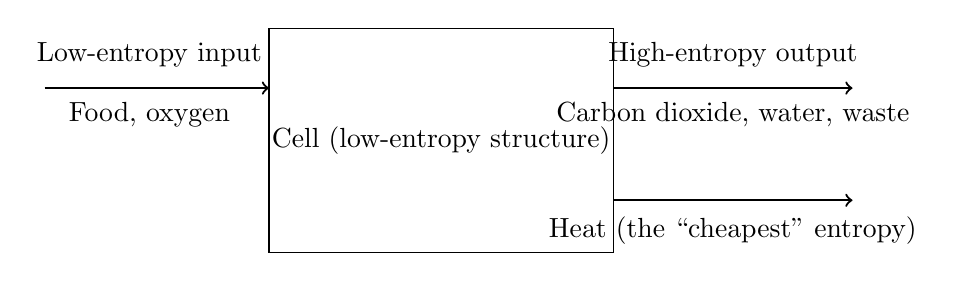
\begin{tikzpicture}[scale=0.95]
\draw (0,0) rectangle (4.6,3);
\node at (2.3,1.5) {Cell (low-entropy structure)};
\draw[->,thick] (-3,2.2) -- (0,2.2);
\node at (-1.6,2.65) {Low-entropy input};
\node at (-1.6,1.85) {Food, oxygen};
\draw[->,thick] (4.6,2.2) -- (7.8,2.2);
\node at (6.2,2.65) {High-entropy output};
\node at (6.2,1.85) {Carbon dioxide, water, waste};
\draw[->,thick] (4.6,0.7) -- (7.8,0.7);
\node at (6.2,0.3) {Heat (the ``cheapest'' entropy)};
\end{tikzpicture}
\end{center}

(This is a human-made representation: the arrows show flows in the matter and energy accounts, not what a cell actually looks like.)

\section{Life's Five Calling Cards}

By now, ``life is an open chemical system that does not violate the second law'' can explain the opening phenomena. But a physicist might ask: waterfalls and flames are open energy flows, too. Are they alive? Clearly not. What distinguishes them? Biologists generally identify five calling cards of life:

\begin{itemize}[itemsep=2pt]
\item \textbf{A boundary}. Life separates itself from its surroundings: a cell has a membrane, and you have skin. Inside the boundary, composition and order differ from those outside, and substances are admitted selectively. A flame has no boundary and disperses in the wind. Chapter 51 explains how the membrane ``guards the gate.''
\item \textbf{Metabolism}. Life continuously carries out chemical reactions: both dismantling (breaking down nutrients and releasing energy) and building (synthesizing its own materials and storing energy). A crystal also ``grows,'' but it merely collects ready-made molecules from solution and piles them on; nothing happens inside it. Chapters 52--55 are devoted to the metabolic network.
\item \textbf{Replication}. Life can copy itself from a set of ``instructions'': a mung bean grows into a plant, which produces new mung beans. Fire can ``spread,'' too, but each spread resembles no particular parent; nothing is being copied. Those instructions---DNA---are the protagonist of Volume III.
\item \textbf{Variation}. Copying occasionally introduces errors, and the environment can also alter the instructions, so offspring differ from their parents. Without variation, the next calling card would be impossible.
\item \textbf{Evolution}. Through selection over successive generations, variations favorable to survival and reproduction are retained, and populations change over time. This is the main thread of the latter half of Volume III. Flames and waterfalls have no ``generations,'' let alone evolution.
\end{itemize}

Together, these five calling cards describe the kind of ``alive'' we recognize. Note that these criteria are \textbf{a descriptive checklist, not a definition carved into nature's stone}. This distinction will matter greatly when we discuss viruses shortly.

\section{The Chemical Machine's Raw Materials}

Calling life a chemical system means providing its list of ingredients. Weigh the atoms in your body: oxygen accounts for just over six-tenths, carbon about two-tenths, hydrogen about one-tenth, and nitrogen about three percent; phosphorus, sulfur, and dozens of other elements together make up only a few percent. But ``little'' does not mean ``unimportant''---screws weigh far less than a car body, too.

\begin{itemize}[itemsep=2pt]
\item \textbf{Water} is not an element, yet it plays the largest role: over six-tenths of your body mass is water. It serves as the cell's solvent, transport medium, and temperature buffer, and participates directly in many reactions. Chapter 23 described its unusual habits---dissolving polar substances, having a high specific heat capacity, and expanding when it freezes. None is wasted; life uses every one.
\item \textbf{Carbon} forms the skeleton of all biological macromolecules. Chapter 36 explained why: carbon atoms can form exactly four covalent bonds and join into chains, rings, and networks, combining stability with variety. Carbohydrates, lipids, proteins, and nucleic acids are all built with carbon.
\item \textbf{Nitrogen} is tucked into proteins and nucleic acids. Air is 78\% nitrogen, but you cannot use a single breath of it directly: \chem{N_2} is too stable. Bacteria and industry must ``break it apart'' into usable forms. This was foreshadowed in Chapter 14 and will return when we discuss material cycles.
\item \textbf{Phosphorus} forms the backbone of two essential pieces of equipment: the ``chain's keel'' in the genetic material DNA, and the energy currency ATP (Chapter 50 will discuss it and clarify what is wrong with the popular expression ``high-energy bond''). Calcium phosphate also supports your bones and teeth.
\item \textbf{Sulfur} has a smaller but indispensable role: some amino acids contain it, and two sulfur atoms can join in a ``disulfide bond,'' stapling a protein's long chain into a fixed shape (Chapter 48). A hair perm works by first undoing and then refastening these sulfur ``staples.''
\item The remaining ``trace elements''---iron, zinc, iodine, magnesium, and others---amount to very little, yet each holds a crucial post: iron at the center of hemoglobin captures oxygen, while magnesium at the center of chlorophyll captures sunlight (Chapter 15).
\end{itemize}

\begin{table}[htbp]
\centering
\begin{tabular}{lll}
\toprule
Player & Main jobs in life & Details \\
\midrule
Water & \shortstack[l]{Solvent, transport, temperature control,\\participation in reactions} & Chapter 23 \\
Carbon & Skeleton of all biological macromolecules & Chapter 36 \\
Nitrogen & Core component of proteins and nucleic acids & Chapter 48 \\
Phosphorus & \shortstack[l]{Backbone of genetic material\\and energy currency} & Chapter 50 \\
Sulfur & ``Staples'' that fix protein shapes & Chapter 48 \\
\bottomrule
\end{tabular}
\caption{Some of life's main players. This table is only an index; later chapters examine them in detail.}
\end{table}

Looking at this list, you can probably sense Parts I--V returning: life invented neither new elements nor new bonds. Working within one small corner of the periodic table, it used rules you already know to build self-maintaining structures.

\section{Writing the Accounts as an Equation}

Now it is time for symbols. The cell's balance of ``low entropy in, high entropy out'' can be written in a familiar language---chemical equations. Taking glucose as an example, the overall balance for cellular respiration is:
\[\chem{C_6H_{12}O_6} + \chem{6O_2} \rightarrow \chem{6CO_2} + \chem{6H_2O}\]

On the left: one structurally complex sugar molecule plus six oxygen molecules. On the right: twelve small, simple molecules, along with released energy. Watch the direction carefully: breaking bonds absorbs energy, and forming bonds releases it (Chapter 27). This overall process releases energy because the new bonds in the products offer a ``better deal'' than those in the reactants. A glucose molecule is concentrated and ordered; dismantling it into a crowd of small molecules and spreading its energy as heat is a broad highway toward increased entropy. This is precisely the ``entropy bill'' the cell pays outward to maintain its own order.

Two cautions are needed immediately. First, this is only the \textbf{overall account}: a cell never lets glucose ``burn up in one go.'' Instead, it divides the process into dozens of controlled steps, gradually ``making change'' from the energy and storing it in ATP. Chapters 52 and 53 will take you through this production line. Second, plant photosynthesis looks at first like the equation written backward, but the two are \textbf{not simply reverse processes}, and the oxygen released comes from water, not carbon dioxide. Chapter 54 will specifically dismantle this common misconception.

\begin{zhengju}
\textbf{A Guinea Pig and Charcoal: The First Weighing of Life's Obedience to Chemistry}

In the late eighteenth century, a view still prevalent in chemistry held that organisms contained a ``vital force,'' so their changes were not bound by the laws of the inorganic world. True or false, the claim needed to be weighed experimentally. In the 1780s, French chemist Lavoisier and mathematician Laplace built an ingenious instrument---the ice calorimeter: a double-walled container with crushed ice between its walls and the test subject in its inner chamber. The subject's heat melted a corresponding amount of ice. Weigh the dripping water, and you had the heat output.

First they put in a guinea pig: over ten hours, it breathed, produced heat, melted considerable ice, and increased the carbon dioxide in the inner chamber's air. Then they replaced it with burning charcoal, carefully weighing it so that combustion produced \textbf{the same amount} of carbon dioxide. Almost the same amount of ice melted. Their conclusion was bold and simple: \textbf{respiration is a kind of slow combustion}. Both consume oxygen, produce carbon dioxide, and release heat, but respiration is much slower and gentler. The heat maintaining body temperature comes not from a mysterious vital force, but from chemical reactions whose accounts can be written as equations.

Parts of this story needed correction, which makes it more credible. Lavoisier thought the ``combustion'' occurred mainly in the lungs; only decades later did people establish that oxidation occurs throughout the body's cells and tissues, with the lungs merely serving as a gas-exchange station. His framework of ``caloric theory'' also had to await the establishment of energy conservation in the 1840s before being fully corrected: heat is not a substance flowing around, but a form of energy. Science works this way: a conclusion can be right before its explanation is complete. Its openness to correction by later evidence is precisely what shows that it is on the right track.

Incidentally, Lavoisier's ice calorimeter provided the first receipt showing that the animal in your home (and you yourself) obeys chemical laws. Over the next two hundred years, activities from muscle contraction to nerve firing were translated, one by one, into accounts of energy and matter. None required an ``exception clause.''
\end{zhengju}

\section{Model Limits and the Awkward Case of Viruses}

When is the model of ``an open system taking in low entropy and exporting entropy'' useful? It explains why you become hungry and warm and need to breathe, why bean sprouts grow, and why wounds heal. It places life firmly within the territory of physical law.

But the model has limits, and a famous awkward customer sits at their edge: the \textbf{virus}.

Check a virus against the five calling cards. Does it have a boundary? A protein coat, and sometimes a stolen piece of membrane---that just about counts. Can it vary and evolve? Very much so: influenza viruses change their faces every year. Can it replicate? Yes---but only by hijacking a host cell's factory; it cannot manufacture a single component itself. The most important card is \textbf{metabolism}. A virus does not eat, drink, breathe, or export entropy. Outside a host, it is a motionless molecular particle that maintains no low-entropy internal order and can remain frozen for years, ``dead but not gone.''

So are viruses alive? The honest answer is: \textbf{it depends on where you draw the passing line on the checklist}. Require ``independent metabolism,'' and viruses are out; require ``replication and evolution,'' and they are in. This is not evasiveness: it shows that ``life'' is a circle humans draw, while nature supplies a continuous gradation. From viruses, viroids (short pieces of nucleic acid), and prions (infectious misfolded proteins), to bacteria and you, the boundaries are inherently blurred. Dormant seeds and cryopreserved cells raise similar questions: with metabolism so low it is almost undetectable, are they ``alive''? A checklist lets you give a reasoned answer; expecting nature to provide a knife-sharp dividing line will disappoint you.

This is the user guide for the chapter's model: it tells you \textbf{how} life operates, but does not decide ``what counts as life.'' The former is a scientific question; the latter is partly a question of definition.

\begin{wuqu}
``The second law says everything becomes disordered, yet life grows more ordered. Therefore life (and evolution) violates natural law and needs a supernatural explanation.''

Counterexamples are right in your kitchen and on your windowsill: water freezes into orderly ice crystals in the refrigerator, and intricate frost patterns grow on window glass in winter. Both are more ``ordered'' than before, yet nobody thinks a miracle is needed, because the refrigerator releases heat outside and the window releases heat to the cold air. Overall entropy keeps increasing. Life is the same: it is an \textbf{open system}, taking in low-entropy food and sunlight and releasing high-entropy waste and heat, while the total entropy of ``organism plus surroundings'' continually increases. From its inception, the second law has governed isolated systems; putting bean sprouts on trial under it misreads the instructions. Incidentally, even ``evolution makes organisms increasingly complex'' is not a requirement of the law. Evolution has no predetermined direction; increasing complexity is a common episode in some local stories, not the universe's goal.
\end{wuqu}

\section{Back to Those Bean Sprouts}

Return to the opening question: which is more disordered, the dried mung beans or the sprouts?

Now we can give a qualified answer. The sprouts' interiors really are more ``ordered'' than a handful of dried beans: cells differentiate, tissues form, and intricate structures develop---local entropy decreases. But half the picture is missing: at every moment, the sprouts absorb water, consume nutrients stored in the beans, take in oxygen, and release carbon dioxide, water vapor, and heat. Treat ``sprouts plus their surroundings'' as a single whole, and entropy increases continuously. Those sprouts that seem to grow ``against disorder'' are actually machines converting stored chemical order into their own structures while exporting large amounts of entropy. They use the same principle as a refrigerator, only a hundred million times more elaborately.

We can also resolve the experiment's little mystery: why do boiled beans grow mold instead of sprouting? Heating destroyed the shapes of the protein machines in their cells (called ``denaturation'' in Chapter 48). Their metabolic factories shut down, and they can no longer present a single calling card. They have declined from an open system into an ordinary heap of organic matter, leaving another set of living open systems---molds---to dismantle them. Chemically, the difference between life and death is \textbf{whether that self-maintaining flow is still running}.

\section{Digging Deeper}

The thread of ``energy flow'' can lead much further. In medicine, high fever and hyperthyroidism are fundamentally problems with the ``valves'' controlling the metabolic fire; measuring basal metabolic rate is like reading this human machine's power meter. In sports science, the heat and heavy sweating you feel while running are the bodily experience of that ``heat expenditure'' in the overall equation. In ecology, an entire food chain can be viewed as a river of energy passed from level to level: grass captures sunlight, sheep eat grass, and wolves eat sheep. At each level, large amounts of energy ``leak'' to the surroundings as heat. This is why food chains usually have only four or five links and top predators are always scarce. Even the origin of life (Chapter 56) cannot escape this framework: the earliest precursors of life may well have arisen in natural energy flows like those at seafloor hydrothermal vents. First there had to be a flow to hitch a ride on; only then could life learn to run its own.

For now, the most natural next question is: what exactly do the food molecules entering a cell look like? Why can carbohydrates serve as fuel, building materials, and even ``identity tags''? Turn to the next chapter, where we begin with the most familiar molecule of all---glucose.

\begin{tiaozhan}
Want to go a level deeper? Chapter 28 introduced the microscopic definition of entropy, Boltzmann's formula $S = k\ln W$, where $W$ is the number of microscopic arrangements available to a system. Viewed this way, a living cell organizes atoms into highly specific arrangements, with a small $W$ and low entropy. Every time it synthesizes such a structure, metabolism must spread more energy into the surroundings, increasing their $W$ by a greater amount. In 1944, physicist Schrödinger presented this idea to the world in his short book \textit{What Is Life?} He coined the term ``negative entropy,'' saying that life ``feeds on negative entropy.'' The phrase is memorable but easily misleading: entropy is not something that can be eaten. Today, the more accurate statement is that life takes in \textbf{free energy} (Chapter 28) and exports entropy. This little book influenced a later generation of physicists who turned to biology, including key figures in the story of DNA's double helix---a story for Volume III. You can skip this box without losing the main thread.
\end{tiaozhan}

\section*{Exercises}

\begin{sikaoti}
\item Draw a ``cellular flow diagram'': use a box for the cell and arrows for matter and energy entering and leaving it, labeling each arrow as low- or high-entropy. Explain in one sentence why the diagram does not violate the second law of thermodynamics.
\item Water in a freezer forms orderly ice crystals (decreasing entropy). Does this violate the second law? State which things must be ``counted together,'' and explain why the back of the refrigerator becomes warm.
\item A bowl of rice provides about 500 kilocalories of energy. Assuming all this energy ultimately enters surroundings at $300\ \mathrm{K}$ as heat, estimate the increase in environmental entropy (use $\Delta S \approx Q/T$ and $1\ \mathrm{kcal}\approx\ud{4.2\times 10^{3}}{J}$). Then express it as ``the equivalent of melting how many kilograms of ice at $0\,^{\circ}\mathrm{C}$?''
\item Check each of the ``five calling cards'' for a campfire, a seed dormant for three years, an influenza virus, and a cryopreserved bacterium. Which cards does each lack? Where do you draw your ``passing line,'' and why?
\item Dried mung beans can remain unchanged for years, while sprouts rot in two or three days. Explain the difference using the three terms ``open system,'' ``water,'' and ``metabolism.''
\item This chapter says, ``Life invented neither new elements nor new bonds; it used old rules to build self-maintaining structures.'' Choose any rule from Volume I (such as energy release on bond formation, shifts in equilibrium, or catalysts) and give an example of life using it.
\end{sikaoti}
